\section{Data Release Production}
\label{sec:drp}

\begin{figure}
\centering
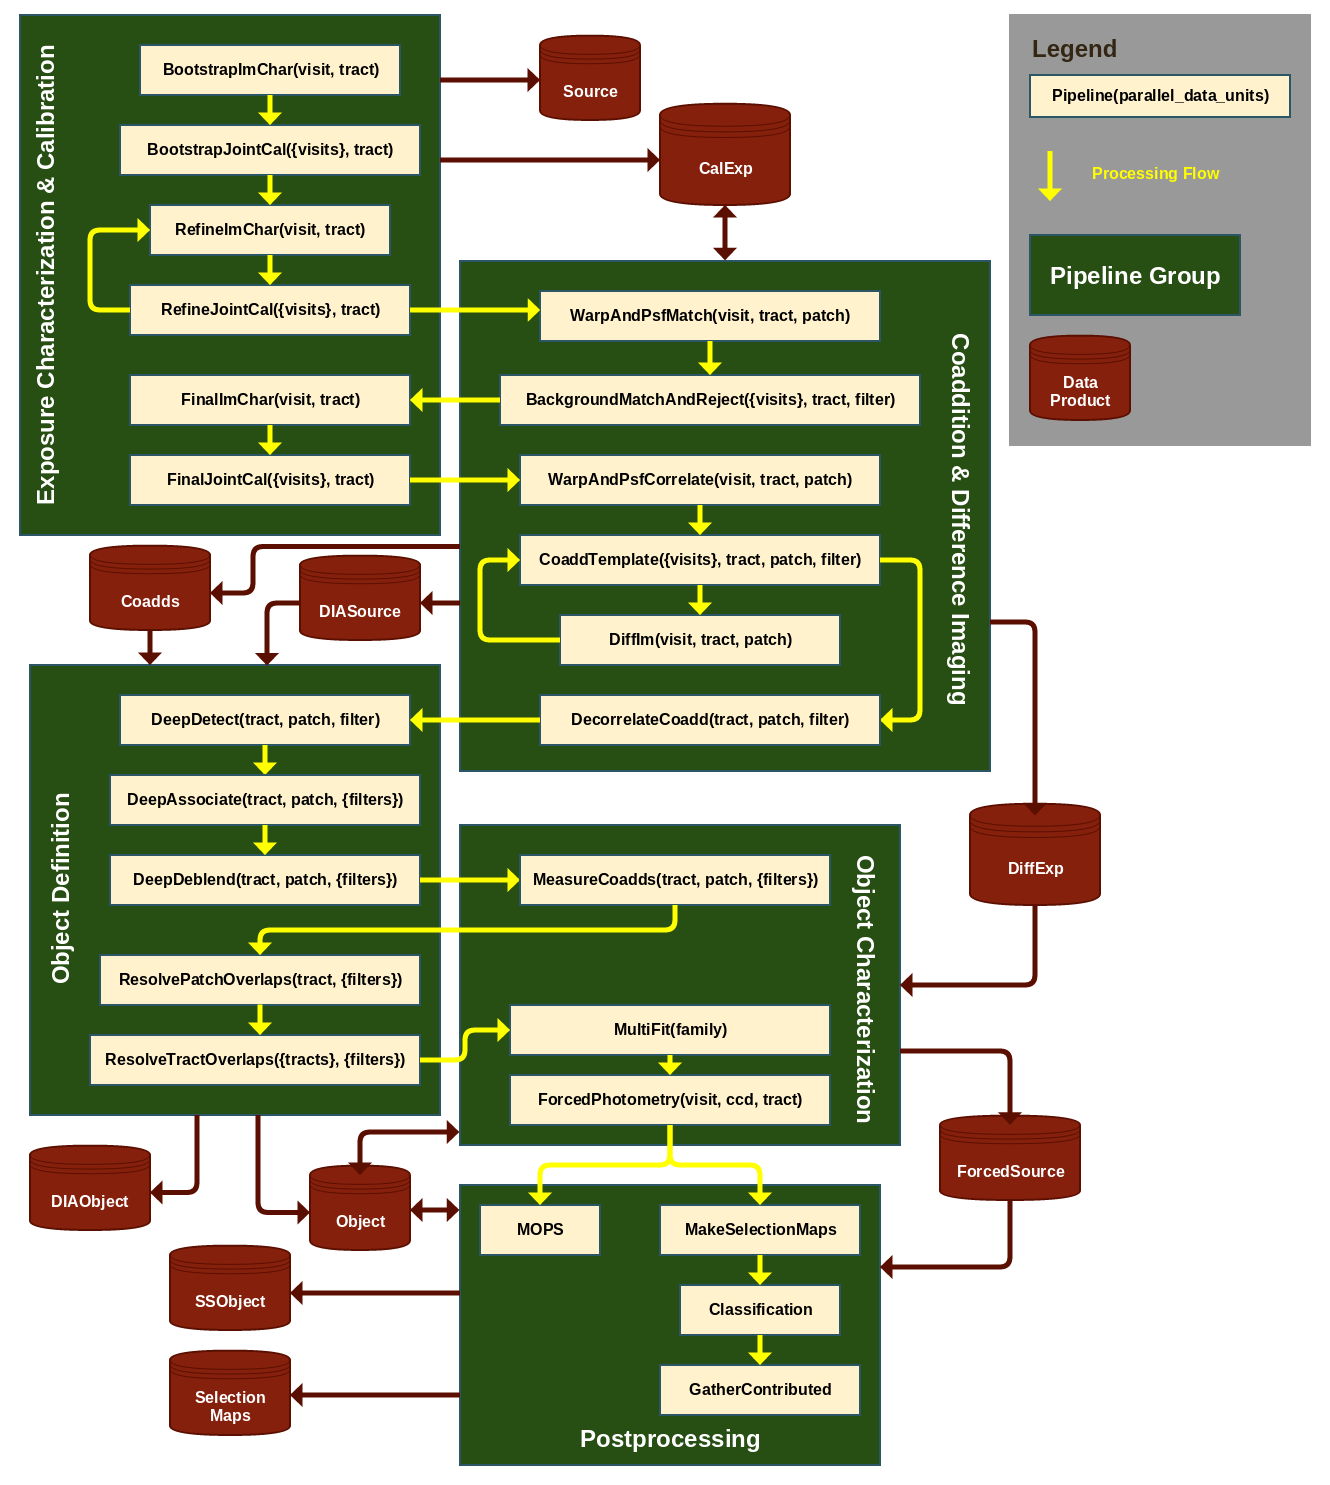
\includegraphics[width=\textwidth]{figures/drp_summary.png}
\caption{Summary of the Data Release Production processing flow.  Processing is split into multiple pipelines, which are conceptually organized into the groups discussed in sections~\ref{sec:drp_imchar_and_jointcal}-\ref{sec:drp_postprocessing}.
\label{fig:drp_summary}}
\end{figure}

A Data Release Production is run every year (twice in the first year of operations) to produce a set of catalog and image data products derived from all observations from the beginning of the survey to the point the production began.  This includes running a variant of the difference image analysis run in Alert Production, in addition to direct analysis of individual exposures and coadded images.  The data products produced by a Data Release Production are summarized in table~\ref{table:drp_data_products}.


\begin{table}
\small
\begin{tabularx}{\textwidth}{ | l | l | X | }
  \hline
  {\bf Name} & {\bf Availability} & {\bf Description} \\
  \hline
  Source & Stored &
  Measurements from direct analysis of individual exposures. \\
  \hline
  DIASource & Stored &
  Measurements from difference imagine analysis of individual exposures. \\
  \hline
  Object & Stored &
  Measurements for a single astrophysical object, derived from all available information, including coadd measurements, simultaneous multi-epoch fitting, and forced photometry.  Does not include solar system objects. \\
  \hline
  DIAObject& Stored &
  Aggregate quantities computing by associating spatially colocated DIASources. \\
  \hline
  ForcedSource & Stored &
  Flux measurements on each direct and difference image at the position of every Object. \\
  \hline
  SSObject & Stored &
  Solar system objects derived by associating DIASources and inferring their orbits. \\
  \hline
  CalExp & Regenerated &
  Calibrated exposure images for each CCD/visit (sum of two snaps). \\
  \hline
  DiffExp & Regenerated &
  Difference between CalExp and PSF-matched template coadd. \\
  \hline
  DeepCoadd & Stored &
  Coadd image with a reasonable combination of depth and resolution. \\
  \hline
  EpochRangeCoadd & Renegerated &
  Coadd image that cover only a limited range of epochs. \\
  \hline
  BestSeeingCoadd & Regenerated &
  Coadd image built from only the best-seeing images. \\
  \hline
  PSFMatchedCoadd & Regenerated &
  Coadd image with a constant, predetermined PSF. \\
  \hline
\end{tabularx}
\caption{Table of public data products produced during a Data Release Production.  A full description of these data products can be found in the Data Products Definition Document (LSE-163).
\label{table:drp_data_products}}
\end{table}

From a conceptual standpoint, data release production can be split into five groups of pipelines, executed in approximately the following order:
\begin{enumerate}
\item We characterize and calibrate each exposure, estimating point-spread functions, background models, and astrometric and photometric calibration solutions.  This iterates between processing individual exposures independently and jointly fitting catalogs derived from multiple overlapping exposures.  These steps are described more fully in section~\ref{sec:drp_imchar_and_jointcal}.
\item We alternately combine images and subtract them, using differences to find artifacts and time-variable sources while building coadds that produce a deeper view of the static sky.  Coaddition and difference imaging is described in section~\ref{sec:drp_coaddition_and_diffim}.
\item We detect and deblend on coadds, while associating these detection with detections from difference imaging to define objects.  We then merge catalogs in the overlap regions between patches and tracts to produce a single contiguous catalog over the full sky.  This is described in section~\ref{sec:drp_object_definition}.
\item We measure objects on coadds and visit-level direct and difference images in object characterization, as described section~\ref{sec:drp_object_characterization}.
\item After all image processing is complete, we run additional catalog-only pipelines to fill in additional object properties.  Unlike previous stages, this postprocessing is not localized on the sky, as it may use statistics computed from the full data release to improve our characterization of individual objects.  Postprocessing pipelines are described in section~\ref{sec:drp_postprocessing}.
\end{enumerate}
This conceptual ordering is an oversimplification of the actual processing flow, however; as shown in Figure~\ref{fig:drp_summary}, pipeline groups are actually interleaved.

Each pipeline in this the diagram represents a particular piece of code excuted in parallel on a specific unit of data, but pipelines may contain additional (and more complex) parallelization to further subdivide that data unit.  The processing flow also includes the possibility of iteration between pipelines, indicated by cycles in the diagram.  The number of iterations in each cycle will be determined (via tests on smaller productions) before the start of the production, allowing us to remove these cycles simply by duplicating some pipelines a fixed number of times.  The final data release production processing can thus be described as a directed acyclic graph (DAG) to be executed by the orchestration middleware, with pipelines as edges and (intermediate) data products as vertices.  Most of the graph will be generated by applications code before the production begins, using a format and/or API defined by the orchestration middleware.  Howver, some parts of the graph must be generated on-the-fly; this will be discussed further in section~\ref{sec:drpMultiFit}.


\subsection{Image Characterization and Calibration}
\label{sec:drp_imchar_and_jointcal}

\begin{note}[ImChar/JointCal Diagram]
Extract ImChar/JointCal pipelines from ``DRP Top-Level Overview'' on confluence and expand detail to show data flow and ordering of ``Task/Process'' boxes.
\end{note}

The first steps in a Data Release Production characterize the properties of individual exposures, by iterating between pixel-level processing of individual visits (``ImChar'', or ``Image Characterization'' steps) and joint fitting of all catalogs overlapping a tract (``JointCal'', or ``Joint Calibration'' steps).  All ImChar steps involve fitting the PSF model and measuring Sources (gradually improving these as we iterate), while JointCal steps fit for new astrometric (WCS) and photometric solutions while building new reference catalogs for the ImChar steps.  Iteration is necessary for a few reasons:
\begin{itemize}
\item The PSF and WCS must have a consistent definition of object centroids.  Celestial positions from a reference catalog are transformed via the WCS to set the positions of stars used to build the PSF model, but the PSF model is then used to measure debiased centroids that feed the WCS fitting.
\item The later stages of photometric calibration and PSF modeling require secure star selection and colors to infer their SEDs.  Magnitude and morphological measurements from ImChar stages are aggregated the reference catalog in the subsequent JointCal stage, allowing these colors and classifications to be used for PSF modeling in the following ImChar stage.
\end{itemize}

The ImChar and JointCal iteration is itself interleaved with background matching, described in section~\ref{sec:drp_coaddition_and_diffim}.  This allows the best backgrounds and masks to be defined in the \hyperref[sec:drpBackgroundMatchAndReject]{BackgroundMatchAndReject} before the final Source measurements, image characterizations, and calibrations.

Each ImChar pipeline runs on a single visit, and each JointCal pipeline runs simultaneously on all visits within a single tract, allowing tracts to be run entirely independently.

The final output data products of the ImChar/JointCal iteration are the Source table and CalExp (calibrated exposure) images.  The latter includes Image, Mask, Variance, Background, PSF, WCS, Calib components that we will track separately.

There are also several intermediate versions of the Source and CalExp data products passed between the ImChar/JointCal pipelines, as well as...

\begin{note}[TODO]
  finish discussing data products.
\end{note}

\subsubsection{BootstrapImChar}
\label{sec:drpBootstrapImChar}

The BootstrapImChar pipeline is the first thing run on each science exposure in a data release.  It has the difficult task of bootstrapping multiple quantities (PSF, WCS, photometric calibration, background model, etc.) that each normally require all of the others to be specified when one is fit.  As a result, while the algorithmic components to be run in this pipeline are generally clear, their ordering and specific requirements are not; algorithms that are run early will have a harder task than algorithms that are run later, and some iteration will almost certainly be necessary.

A plausible (but by no means certain) high-level algorithm for this pipeline is given below in pseudocode.  Highlighted terms are described in more detail below the pseudocode block.

\lstset{
    language=Python,
    basicstyle=\scriptsize\ttfamily,
    keywordstyle=\bfseries,
    commentstyle=\color{darkgray},
    escapeinside={\%}{\%},
}

% Define a local macro that lets us refer to sections of the text
% more easily (will undefine at the end of this section).
\newcommand{\hr}[1]{\hyperref[sec:drpBootstrapImChar_#1]{#1}}

\begin{lstlisting}
def BootstrapImChar(%\hr{raw}%, %\hr{reference}%):
    # Some data products components are visit-wide and some are per-CCD;
    # these imaginary data types lets us deal with both.
    # VisitExposure also has components; most are self-explanatory, and
    # {mi} == {image,mask,variance} (for "MaskedImage").
    calexp = VisitExposure()
    sources = VisitCatalog()
    snaps = VisitMaskedImageList()  # holds both snaps, but only {image,mask,variance}
    parallel for ccd in ALL_SENSORS:
        snaps[ccd] = [%\hr{RunISR}%(raw[ccd]) for snap in SNAP_NUMBERS]
        snaps[ccd].mask = %\hr{SubtractSnaps}%(snaps[ccd])
        calexp[ccd].mi = %\hr{CombineSnaps}%(snaps[ccd])
    calexp.psf = %\hr{FitWavefront}%(calexp[WAVEFRONT_SENSORS].mi)
    calexp.{image,mask,variance,background}
        = %\hr{SubtractBackground}%(calexp.mi)
    parallel for ccd in ALL_SENSORS:
        sources[ccd] = %\hr{DetectSources}%(calexp.{mi,psf})
    sources[ccd] = %\hr{DeblendSources}%(sources[ccd], calexp.{mi,psf})
    sources[ccd] = %\hr{MeasureSources}%(sources[ccd], calexp.{mi,psf})
    matches = %\hr{MatchSemiBlind}%(sources, reference)
    while not converged:
        %\hr{SelectStars}%(matches, exposures)
        calexp.wcs = %\hr{FitWCS}%(matches, sources, reference)
        calexp.psf = %\hr{FitPSF}%(matches, sources, calexp.{mi,wcs})
        %\hr{WriteDiagnostics}%(snaps, calexp, sources)
        parallel for ccd in ALL_SENSORS:
            snaps[ccd] = %\hr{SubtractSnaps}%(snaps[ccd], calexp[ccd].psf)
            calexp[ccd].mi = %\hr{CombineSnaps}%(snaps[ccd])
            calexp[ccd].mi = %\hr{SubtractStars}%(calexp[ccd].{mi,psf}, sources[ccd])
        calexp.{mi,background} = %\hr{SubtractBackground}%(calexp.mi)
        parallel for ccd in ALL_SENSORS:
            sources[ccd] = %\hr{DetectSources}%(calexp.{mi,psf})
            calexp[ccd].mi, sources[ccd] =
                %\hr{ReinsertStars}%(calexp[ccd].{mi,psf}, sources[ccd])
            sources[ccd] = %\hr{DeblendSources}%(sources[ccd], calexp.{mi,psf})
            sources[ccd] = %\hr{MeasureSources}%(sources[ccd], calexp.{mi,psf})
        matches = %\hr{MatchNonBlind}%(sources, reference)
    calexp.psf.apcorr = %\hr{FitApCorr}%(matches, sources)
    parallel for ccd in SCIENCE_SENSORS:
        sources[ccd] = %\hr{ApplyApCorr}%(sources[ccd], calexp.psf)
    return calexp, sources
\end{lstlisting}

\paragraph{Input Data Product: Raw}
\label{sec:drpBootstrapImChar_raw}

Raw amplifier images from science and wavefront CCDs, spread across one or more snaps.  Needed telescope telemetry (seeing estimate, approximate pointing) is assumed to be included in the raw image metadata.

\paragraph{Input Data Product: Reference}
\label{sec:drpBootstrapImChar_reference}

A full-sky catalog of reference stars derived from both external (e.g. Gaia) and LSST data.

The \hyperref[sec:drpInitialJointCal]{InitialJointCal} pipeline will later define a deeper reference catalog derived from this one and the new data being processed, but the origin and depth of the initial reference catalog is largely TBD.  It will almost certainly include Gaia stars, but it may also include data from other telescopes, LSST special programs, LSST commissioning observations, and/or the last LSST data release.

\paragraph{Output Data Product: Source}
\label{sec:drpBootstrapImChar_sources}

A preliminary version of the Source table.  This could contain all of the columns in the DPDD Source schema if the \hr{MeasureSources} is appropriately configured, but some of these columns are likely unnecessary in its role as an intermediate data product that feeds \hyperref[sec:drpInitialJointCal]{InitialJointCal}, and it is likely that other non-DPDD columns will be present for that role.

BootstrapImChar also has the capability to produce even earlier versions of the Source table for diagnostic purposes (see \hr{WriteDiagnostics}).  These tables are not associated with any photometric calibration or aperture correction, and some may not have any measurements besides centroids, and hence are never substitutable for the final Source table.

\paragraph{Output Data Product: CalExp}
\label{sec:drpBootstrapImChar_calexp}

A preliminary version of the CalExp (calibrated direct exposure).  CalExp is an \hyperref[sec:spImagesExposure]{Exposure} object, and hence it has several components.  BootstrapImChar is the only pipeline that actually updates all of them.  Some CalExp components are determined at the scale of a full FoV and hence should probably be persisted at the visit level (PSF, WCS, Calib, Background), while others are straightforward CCD-level data products (Image, Mask, Variance).

\paragraph{RunISR}
\label{sec:drpBootstrapImChar_RunISR}

Delegate to the \hyperref[sec:acISR]{ISR algorithmic component} to perform standard detrending as well as brighter-fatter correction and interpolation for pixel-area variations (\hyperref[sec:acFixPixelAreaVariations]{Warping Irregularly-Sampled Images}).  It is possible that these corrections will require a PSF model, and hence must be backed-out and recorrected at a later stage when an improved PSF model is available.

We assume that the applied flat field is appropriate for background estimation.

\paragraph{SubtractSnaps}
\label{sec:drpBootstrapImChar_SubtractSnaps}

Delegate to the \hyperref[sec:acSnapSubtraction]{Snap Subtraction algorithmic component} to mask artifacts in the difference between snaps.  If passed a PSF (as in the second call), also interpolate them by delegating to the \hyperref[sec:acArtifactInterpolation]{Artifact Interpolation} algorithmic component.

We assume here that the PSF modeled on the combination of the two Snaps is sufficient for interpolation on the Snaps individually; if this is not true, we can just mask and interpolate both Snaps when an artifact appears on either of them (or we could do per-Snap PSF estimation, but that's a lot more work for very little gain).

\paragraph{CombineSnaps}
\label{sec:drpBootstrapImChar_CombineSnaps}

Delegate to the \hyperref[sec:acCoaddition]{Image Coaddition algorithmic component} to combine the two Snaps while handling masks appropriately.

We assume there is no warping involved in combining snaps.  If this is needed, we should instead advocate for dropping snaps in favor of a a single longer exposure.

\paragraph{FitWavefront}
\label{sec:drpBootstrapImChar_FitWavefront}

Delegate to the \hyperref[sec:acWavefrontSensorPSF]{Wavefront Sensor PSF algorithmic component} to generate an approximate PSF using only data from the wavefront sensors and observational metadata (e.g. reported seeing).

Processing the wavefront sensors will likely require some form of detection and measurement; we currently consider this to be part of the \hyperref[sec:acWavefrontSensorPSF]{Wavefront Sensor PSF} code, though it may delegate to e.g. \hyperref[sec:acSourceDetection]{Source Detection} and/or \hyperref[sec:acSingleVisitMeasurement]{Single Visit Measurement}.

The required quality of this PSF estimate is TBD (requirements are likely to come from crowded fields), and it is possible that a simple circular profile with the appropriate seeing may suffice.  Robustness to poor data quality and crowding is much more important than accuracy.

\paragraph{SubtractBackground}
\label{sec:drpBootstrapImChar_SubtractBackground}

Delegate to the \hyperref[sec:acBackgroundEstimation]{Background Estimation} algorithmic component to model and subtract the background consistently over the full field of view.

The multiple backgrounds subtracted in BootstrapImChar may or may not be cumulative (i.e. we may or may not add the previous background back in before estimating the latest one).

\paragraph{DetectSources}
\label{sec:drpBootstrapImChar_DetectSources}

Delegate to the \hyperref[sec:acSourceDetection]{Source Detection algorithmic component} to find above-threshold regions (\hyperref[sec:spFootprints]{Footprints}) and peaks within them in a PSF-correlated version of the image.

In crowded fields, each iteration of detection will decrease the threshold, increasing the number of objects detection.  Because this will treat fluctuations in the background due to undetected objects as noise, we may need to extend PSF-correlation to the appropriate filter for an image with correlated noise and characterize the noise field from the image itself.

Because we will use wavefront data to constrain the PSF, we also run detection on the wavefront sensors.  It is possible that this will require a different algorithmic component if we cannot just treat the wavefront sensors as science sensors with an out-of-focus PSF.

\paragraph{DeblendSources}
\label{sec:drpBootstrapImChar_DeblendSources}

Delegate to the \hyperref[sec:acSingleVisitDeblending]{Single Visit Deblending algorithmic component} to split \hyperref[sec:spFootprints]{Footprints} with multiple peaks into deblend families.

Because we will use wavefront data to constrain the PSF, we also run deblending on the wavefront sensors.  It is possible that this will require a different algorithmic component if we cannot just treat the wavefront sensors as science sensors with an out-of-focus PSF, and we need deblending to extract wavefront information.

\paragraph{MeasureSources}
\label{sec:drpBootstrapImChar_MeasureSources}

Delegate to the \hyperref[sec:acSingleVisitMeasurement]{Single Visit Measurement algorithmic component} to measure source properties.

In BootstrapImChar, we anticipate using the \hyperref[sec:acReplaceNeighborsWithNoise]{Neighbor Noise Replacement} approach to deblending, with the following plugin algorithms:
\begin{itemize}
\item \hyperref[sec:acCentroidAlgorithms]{Centroids}
\item \hyperref[sec:acShapeAlgorithms]{Second-Moment Shapes}
\item \hyperref[sec:acPixelFlags]{Pixel Flag Aggregation}
\item \hyperref[sec:acAperturePhotometry]{Aperture Photometry} (but only for one or two radii)
\item \hyperref[sec:acStaticPointSourceModels]{Static Point Source Models}
\end{itemize}

Because we will use wavefront data to constrain the PSF, we also run measurement on the wavefront sensors (but probably without any flux measurement algorithms, and perhaps with modified versions of other algorithms).  It is possible that this will require a different algorithmic component if we cannot just treat the wavefront sensors as science sensors with an out-of-focus PSF.

\paragraph{MatchSemiBlind}
\label{sec:drpBootstrapImChar_MatchSemiBlind}

Delegate to the \hyperref[sec:acSingleVisitReferenceMatching]{Single Visit Reference Matching algorithmic component} to match source catalogs to a global reference catalog.  This occurs over the full field of view, ensuring robust matching even when some CCDs have no matchable stars due to crowding, flux limits, or artifacts.

``Semi-Blind'' refers to the fact that the WCS is not yet well known (all we have is what is provided by the observatory), so the matching algorithm must account for an unknown (but small) offset between the WCS-predicted sources positions and the reference catalog positions.

\paragraph{SelectStars}
\label{sec:drpBootstrapImChar_SelectStars}

Use reference catalog classifications and source flags to select a clean sample stars to use for later stages.

If we decide not to rely on a pre-existing reference catalog to separate stars from galaxies and other objects, we will need a new algorithmic component to select stars based on source measurements.

\paragraph{FitWCS}
\label{sec:drpBootstrapImChar_FitWCS}

Delegate to the \hyperref[sec:acSingleVisitAstrometricFit]{Single Visit Astrometric Fit algorithmic component} to determine the WCS of the image.

We assume this works by fitting a simple mapping from the visit's focal plane coordinate system to the sky and composing it with the (presumed fixed) mapping between CCD coordinates and focal plane coordinates.  This fit will be improved in later pipelines, so it does not need to be exact; $<$0.05 arcsecond accuracy should be sufficient.

As we iterate in crowded fields, the number of degrees of freedom in the WCS should be allowed to slowly increase.

\paragraph{FitPSF}
\label{sec:drpBootstrapImChar_FitPSF}

Delegate to the \hyperref[sec:acFullVisitPSF]{Full Visit PSF Modeling algorithmic component} to construct an improved PSF model for the image.

Because we are relying on a reference catalog to select stars, we should be able to use colors from the reference catalog to estimate SEDs an include wavelength dependence in the fit.  If we do not use a the reference catalog early in BootstrapImChar, PSF estimation here will not be wavelength-dependent.  In either case the PSF model will be further improved in later pipelines.

PSF estimation at this stage must include some effort to model the wings of bright stars, even if this is tracked and constrained separately from the model for the core of the PSF.

As we iterate in crowded fields, the number of degrees of freedom in the PSF model should be allowed to slowly increase.

\paragraph{WriteDiagnostics}
\label{sec:drpBootstrapImChar_WriteDiagnostics}

If desired, the current state of the \texttt{source}, \texttt{calexp}, and \texttt{snaps} variables may be persisted here for diagnostic purposes.

\paragraph{SubtractStars}
\label{sec:drpBootstrapImChar_SubtractStars}

Subtract all detected stars above a flux limit from the image, using the PSF model.  In crowded fields, this should allow subsequent \hr{SubtractBackground} and \hr{DetectSources} steps to push fainter by removing the brightest stars in the image.

Sources classified as extended are never subtracted.

\paragraph{ReinsertStars}
\label{sec:drpBootstrapImChar_ReinsertStars}

Add stars removed in \hr{SubtractStars} back into the image, and merge corresponding \hyperref[sec:spFootprints]{Footprints} and peaks into the source catalog.

\paragraph{MatchNonBlind}
\label{sec:drpBootstrapImChar_MatchNonBlind}

Match a single-CCD source catalog to a global reference frame, probably by delegating to \hyperref[sec:acJointCalMatching]{the same matching algorithm used in JointCal pipelines}.  A separate algorithm component may be needed for efficiency or code maintenance reasons; this is a simple limiting case of the multi-way JointCal matching problem that may or may not merit a separate simpler implementation.

``Non-Blind'' refers to the fact that the WCS is now known well enough that there is no significant offset between WCS-projected source positions and reference catalog positions.

\paragraph{FitApCorr}
\label{sec:drpBootstrapImChar_FitApCorr}

Delegate to the \hyperref[sec:acApCorr]{Aperture Correction algorithmic component} to construct a curve of growth from aperture photometry measurements and build an interpolated mapping from other fluxes to the predicted integrated flux at infinity.

\paragraph{ApplyApCorr}
\label{sec:drpBootstrapImChar_ApplyApCorr}

Delegate to the \hyperref[sec:acApCorr]{Aperture Correction algorithmic component} to apply aperture corrections to flux measurements.

% Undeclare the local hyperref macro
\let\hr\undefined

\subsubsection{InitialJointCal}
\label{sec:drpInitialJointCal}

In InitialJointCal, we jointly process all of the Source tables produced by running \hyperref[sec:drpBootstrapImChar]{BootstrapImChar} on each visit in a tract.  There are four steps:
\begin{enumerate}
\item We match all sources and the reference catalog by delegating to \hyperref[sec:acJointCalMatching]{JointCalMatching}.  This is a non-blind search; we assume the WCSs output by BootstrapImChar are good enough that we don't need to fit for any additional offsets between images at this stage.  Some matches will not include a reference object, as the sources will almost certainly extend deeper than the reference catalog.
\item We classify matches to select a clean sample of low-variability stars for later steps, delegating to \hyperref[sec:acJointCalClassification]{JointCalClassification}.  This uses morphological and possibly color information from source measurements as well as reference catalog information (where available).  This step also assigns an inferred SED to each match from its colors; for matches associated with a reference object, whether this supersedes SEDs or colors in the reference catalog is TBD.
\item We fit simultaneously for improved astrometric solution by requiring each star in a match to have the same position.  This may need to correct (perhaps approximately) for centroid shifts due to DCR and/or proper motion; if it does not, it must be robust against these shifts (perhaps via outlier rejection).  The models and parameters to fit are TBD in detail, but they will represent further perturbation of the WCS fit in BootstrapImChar.  This fit generates a new WCS component for each CalExp.
\item We fit simultaneously for photometric zeropoints by requiring each star in a match to have the same flux after applying smoothed monochromatic flat fields produced by the calibration products pipeline.  There is a small chance this fit will also be used to further constrain those monochromatic flat fields.  This fit generates a new PhotoCalib component for each CalExp.
\end{enumerate}

In addition to updating the CalExp WCS and PhotoCalib, InitialJointCal generates a new Reference dataset containing the joint-fit centroids and fluxes for each of its match groups as well as their classifications and inferred SEDs.

\subsubsection{RefineImChar}
\label{sec:drpRefineImChar}

RefineImChar performs an incremental improvement on the measurements and PSF model produced by \hyperref[sec:drpBootstrapImChar]{BootstrapImChar}, using the improved reference catalog, WCS, and PhotoCalib produced by \hyperref[sec:drpInitialJointCal]{InitialJointCal}.  Its steps are thus a strict subset of those in \hyperref[sec:drpBootstrapImChar]{BootstrapImChar}.  A pseudocode description of RefineImChar is given below, but all steps refer to back to the descriptions in \ref{sec:drpBootstrapImChar}:

\newcommand{\hr}[1]{\hyperref[sec:drpBootstrapImChar_#1]{#1}}

\begin{lstlisting}
def RefineImChar(%\hr{calexp}%, %\hr{sources}%, %\hr{reference}%):
    matches = %\hr{MatchNonBlind}%(sources, reference)
    %\hr{SelectStars}%(matches, exposures)
    calexp.psf = %\hr{FitPSF}%(matches, sources, calexp.{mi,wcs})
    parallel for ccd in ALL_SENSORS:
        calexp[ccd].mi = %\hr{SubtractStars}%(calexp[ccd].{mi,psf}, sources[ccd])
    calexp.{mi,background} = %\hr{SubtractBackground}%(calexp.mi)
    parallel for ccd in ALL_SENSORS:
        sources[ccd] = %\hr{DetectSources}%(calexp.{mi,psf})
        calexp[ccd].mi, sources[ccd] =
            %\hr{ReinsertStars}%(calexp[ccd].{mi,psf}, sources[ccd])
        sources[ccd] = %\hr{DeblendSources}%(sources[ccd], calexp.{mi,psf})
        sources[ccd] = %\hr{MeasureSources}%(sources[ccd], calexp.{mi,psf})
    calexp.psf.apcorr = %\hr{FitApCorr}%(matches, sources)
    parallel for ccd in ALL_SENSORS:
        sources[ccd] = %\hr{ApplyApCorr}%(sources[ccd], calexp.psf)
    return calexp, sources
\end{lstlisting}

This is essentially just another iteration of the loop in in \hyperref[sec:drpBootstrapImChar]{BootstrapImChar}, without the WCS-fitting or artifact-handling stages.

Note that RefineImChar does not update the CalExp's WCS, PhotoCalib, Image, or Variance (and its Mask is only updated to indicate new detections).

% Undeclare the local hyperref macro
\let\hr\undefined

\subsubsection{FinalImChar}
\label{sec:drpFinalImChar}



\subsubsection{FinalJointCal}
\label{sec:drpFinalJointCal}

\subsection{Coaddition and Difference Imaging}
\label{sec:drp_coaddition_and_diffim}

\begin{note}[Coaddition, DiffIm Diagram]
Extract Coaddition and DiffIm pipelines from ``DRP Top-Level Overview'' on confluence and expand detail to show data flow and ordering of ``Task/Process'' boxes.
\end{note}

\subsubsection{WarpAndPsfMatch}
\label{sec:drpWarpAndPsfMatch}
\subsubsection{BackgroundMatchAndReject}
\label{sec:drpBackgroundMatchAndReject}
\subsubsection{WarpAndPsfCorrelate}
\label{sec:drpWarpAndPsfCorrelate}
\subsubsection{CoaddTemplate}
\label{sec:drpCoaddTemplate}
\subsubsection{DiffIm}
\label{sec:drpDiffIm}
\subsubsection{DecorrelateCoadds}
\label{sec:drpDecorrelateCoadds}

\subsection{Object Definition}
\label{sec:drp_object_definition}

\begin{note}[Detection/Association/Deblending Diagram]
Extract process\_coadds pipeline from ``DRP Top-Level Overview'' on confluence and expand detail to show data flow and ordering of ``Task/Process'' boxes.
\end{note}

\subsubsection{DeepDetect}
\label{sec:drpDeepDetect}
\subsubsection{DeepAssociate}
\label{sec:drpDeepAssociate}
\subsubsection{DeepDeblend}
\label{sec:drpDeepDeblend}
\subsubsection{ResolvePatchOverlaps}
\label{sec:drpResolvePatchOverlaps}
\subsubsection{ResolveTractOverlaps}
\label{sec:drpResolveTractOverlaps}

\subsection{Object Characterization}
\label{sec:drp_object_characterization}

\begin{note}[Object Characterization Diagram]
Extract multifit/forced\_photometry pipelines from ``DRP Top-Level Overview'' on confluence and expand detail to show data flow and ordering of ``Task/Process'' boxes.
\end{note}

\subsubsection{MeasureCoadds}
\label{sec:drpMeasureCoadds}
\subsubsection{MultiFit}
\label{sec:drpMultiFit}
\subsubsection{ForcedPhotometry}
\label{sec:drpForcedPhotometry}

\subsection{Postprocessing}
\label{sec:drp_postprocessing}

\begin{note}[Postprocessing Diagram]
Extract Afterburner pipelines from ``DRP Top-Level Overview'' on confluence and expand detail to show data flow and ordering of ``Task/Process'' boxes.
\end{note}

\subsubsection{MOPS}
\label{sec:drpMOPS}
\subsubsection{MakeSelectionMaps}
\label{sec:drpMakeSelectionMaps}
\subsubsection{Classification}
\label{sec:drpClassification}
\subsubsection{GatherContributed}
\label{sec:drpGatherContributed}

\subsection{UNCAPTURED DEPENDENCIES}

\begin{itemize}
\item Where does the initial reference catalog at the start of the DRP come from?  This could require special observations in commissioning or before the start of the survey, as well as addition algorithms and software.  If DRP always uses a reference catalog for star selection in ImChar, we need to actually do the classification for that at some point.
\item How do we test all of the wavelength-dependent photometric calibration and PSF stuff on precursor data?  Are we going to characterize DECam well enough to just use it directly, or do we need to mock things up or rely more on JointCal?
\end{itemize}

